\definecolor{r1}{RGB}{86,16,16};
\definecolor{r2}{RGB}{151,28,28};
\definecolor{r3}{RGB}{214,39,40};
\definecolor{r4}{RGB}{227,104,104};
\definecolor{r5}{RGB}{239,169,169};
\definecolor{b1}{RGB}{11,43,65};
\definecolor{b2}{RGB}{22,86,131};
\definecolor{b3}{RGB}{31,119,180};
\definecolor{b4}{RGB}{59,154,222};
\definecolor{b5}{RGB}{124,188,233};
\definecolor{g1}{RGB}{16,60,16};
\definecolor{g2}{RGB}{33,120,33};
\definecolor{g3}{RGB}{49,180,49};
\definecolor{g4}{RGB}{95,211,95};
\definecolor{g5}{RGB}{135,222,135};
\definecolor{p1}{RGB}{39,23,53};
\definecolor{p2}{RGB}{77,47,106};
\definecolor{p3}{RGB}{116,70,160};
\definecolor{p4}{RGB}{148,103,189};
\definecolor{p5}{RGB}{179,149,208};
\definecolor{tab_orange}{RGB}{255,127,14};
\definecolor{tab_blue}{RGB}{31, 119, 180};
\definecolor{mixed_color}{RGB}{143, 123, 97}
\definecolor{tab_brown}{RGB}{140,86,75};


\begin{tikzpicture}

\node at (-7.5,11.6) {{\fontfamily{phv}\scalebox{1}{\fontsize{8pt}{0pt}\selectfont{A}}}};

\node at (-4.7,11.6) {{\fontfamily{phv}\scalebox{1}{\fontsize{7pt}{0pt}\selectfont \parbox{4.5cm} {\hyphenpenalty=10000\exhyphenpenalty=10000\raggedright
Age distribution of healthy controls
}}}};
\node[inner sep=0pt] (russell) at (-4,8.5) {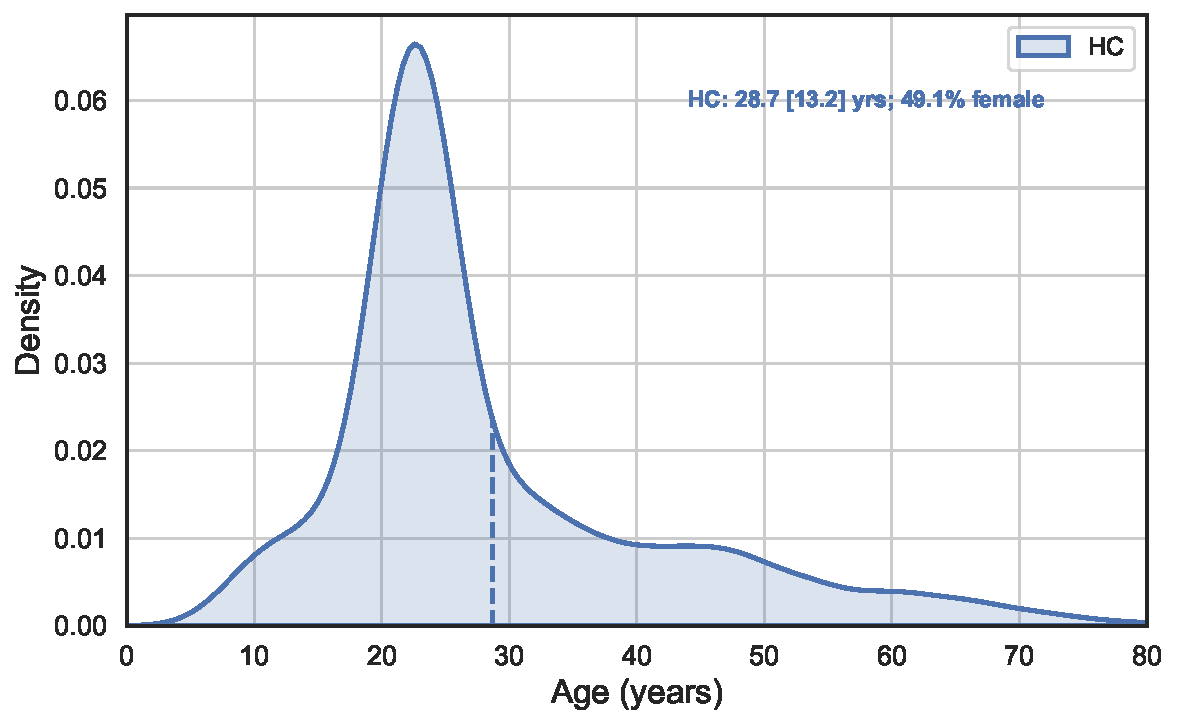
\includegraphics[width=0.35\textwidth]{fig1.pdf}};












\node at (0.4,11.6) {{\fontfamily{phv}\scalebox{1}{\fontsize{8pt}{0pt}\selectfont{B}}}};

\node at (3.2,11.6) {{\fontfamily{phv}\scalebox{1}{\fontsize{7pt}{0pt}\selectfont \parbox{4.5cm} {\hyphenpenalty=10000\exhyphenpenalty=10000\raggedright
Proportion of data modalities 
}}}};
\node[inner sep=0pt] (russell) at (2.9,8.83) {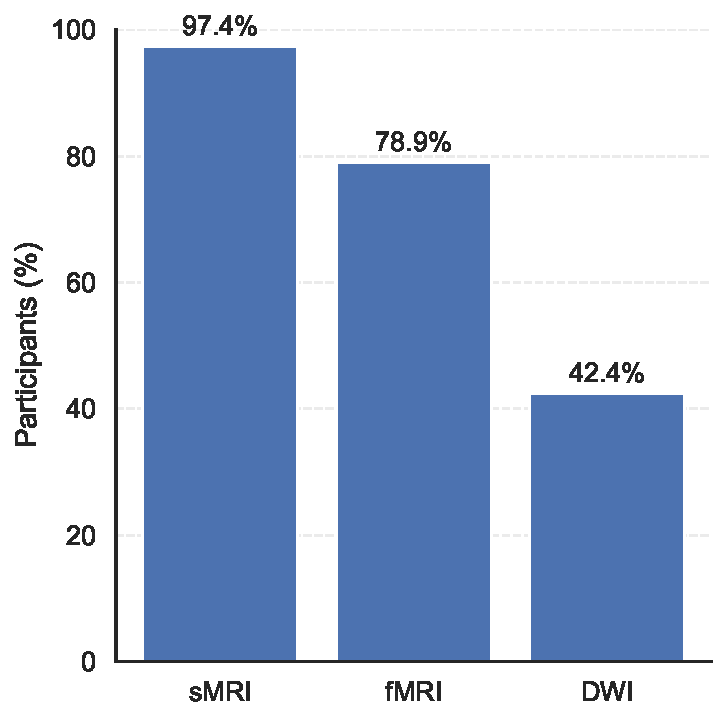
\includegraphics[width=0.23\textwidth]{fig2.pdf}};





\end{tikzpicture}